% !TeX spellcheck = de_DE
\section{Lunar Lander}
Die vorherigen Kapiteln beschreiben die Ergebnisse des parallelisierten Verfahrens. Mit $40$ Prozessen wird ein \emph{SpeedUp} für die \emph{EvaluationTime} von $26.7$ und $29.6$ gemessen. Allerdings erfüllen die in diesen Umgebungen optimierten \ac{KNN} nicht die Eigenschaft der Generalisierung. Jedes \ac{KNN} beginnt die Evaluation immer in derselben Startposition und hat dafür gute Optimierungsergebnisse erzielt. Würden diese \ac{KNN} in einer Umgebung mit einer abweichenden Startposition starten, besteht eine hohe Wahrscheinlichkeit, dass nicht das gewünschte Ergebnis erreicht wird. Bei der durchgeführten Analyse wird eine generelle Lösung für alle Startpositionen nicht benötigt und ist zusätzlich durch die hohen benötigten Trainingszeiten ungeeignet. In diesem Kapitel wird ein letztes Optimierungsproblem aus dem OpenAI Gym mit dem Namen \emph{Lunar Lander} vorgestellt. Dieses Beispiel zeigt, wie eine generelle Lösung für alle Startsituation entwickelt werden kann und was die hierfür benötigten Laufzeiten sind. Das Verfahren wird nur mit der parallelisierten Algorithmus durchgeführt, aber mit den zuvor gemessenen \emph{SpeedUp} Werte lässt sich auf die Laufzeit des sequenziellen Verfahrens schließen.
\begin{figure}[!h]
	\centering
	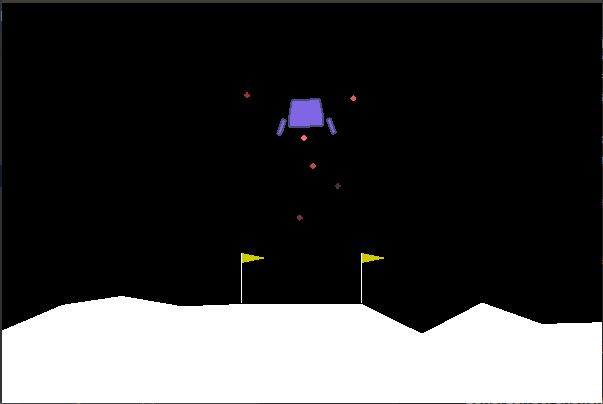
\includegraphics[width=0.5\textwidth]{./img/lunar_lander_env.JPG} 
	\caption{Darstellung der \emph{Lunar Lander} Umgebung aus dem OpenAI Gym}
	\label{fig:lunar_lander_env}
\end{figure} 
\\\\
Abbildung \ref{fig:lunar_lander_env} zeigt eine Raumschiff und eine Landeplattform, die sich zwischen den zwei Fahnen befindet. Ziel der Umgebung ist das Landen des Raumschiffs auf dieser. Für das Optimierungsproblem stehen insgesamt $8$ Eingabewerte zur Verfügung, welche die Position, Geschwindigkeit und den Winkel das Raumschiffs beschreiben. Die Koordinaten der Landeplattform sind nicht enthalten, da sich diese immer an derselben Position befindet. Als Aktion kann entweder die Hauptdüse unten oder eine Steuerdüsen links bzw. rechts des Raumschiffs aktiviert werden. Ebenfalls ist es möglich gar keinen Antrieb zu aktivieren. Die Simulation der Umgebung wird beendet, wenn das Raumschiff entweder abstürzt oder erfolgreich landet. Wie die anderen Umgebungen des OpenAI Gyms wird für jeden Zeitschritt ein \emph{reward} vergeben. Diese werden während der Simulation summiert und bilden den Fitnesswert. Einen positiven \emph{reward} gibt es, wenn das Raumschiff sinkt und sich der Plattform annähert. Zusätzlich gibt es einen Bonus, wenn das Raumschiff sich im Ziel befindet oder die Landefüße den Boden berühren. Für jeden Zeitschritt, in welchem ein Antrieb aktiviert ist, wird ein kleiner Betrag vom \emph{reward} subtrahiert. Somit muss für die Maximierung des Fitnesswertes das Raumschiff so wenig Treibstoff wie möglich verbrauchen. Im Falle eines Absturzes, gibt es einen negativen \emph{reward}.
\\\\
Für die Optimierung werden die Parameter der \emph{Pendulum} Umgebung übernommen. Somit steht eine Population von $1000$ Agenten zur Verfügung. Jedes \ac{KNN} besitzt entsprechend der Ein- und Ausgabewerte acht \emph{Input}- und vier \emph{Output}-Neuronen. Das Optimierungsproblem ist so konfiguriert, dass die Startzustände zufällig gewählt werden. Um eine generelle Lösungsstrategie zu finden muss jeder Agent zehn Durchläufe in der Umgebung absolvieren. Für den finalen Fitnesswert werden die Ergebnisse der einzelnen Durchläufe summiert. Das Verfahren wird beendet, wenn ein Agent in jedem der zehn Durchläufen einen Fitnesswert von über $200$ Punkten erreicht. So ist sichergestellt, dass der Agent auf verschiedene Startsituationen entsprechend reagieren kann.
\begin{figure}[!h]
	\centering
	\begin{minipage}[]{0.49\textwidth}
		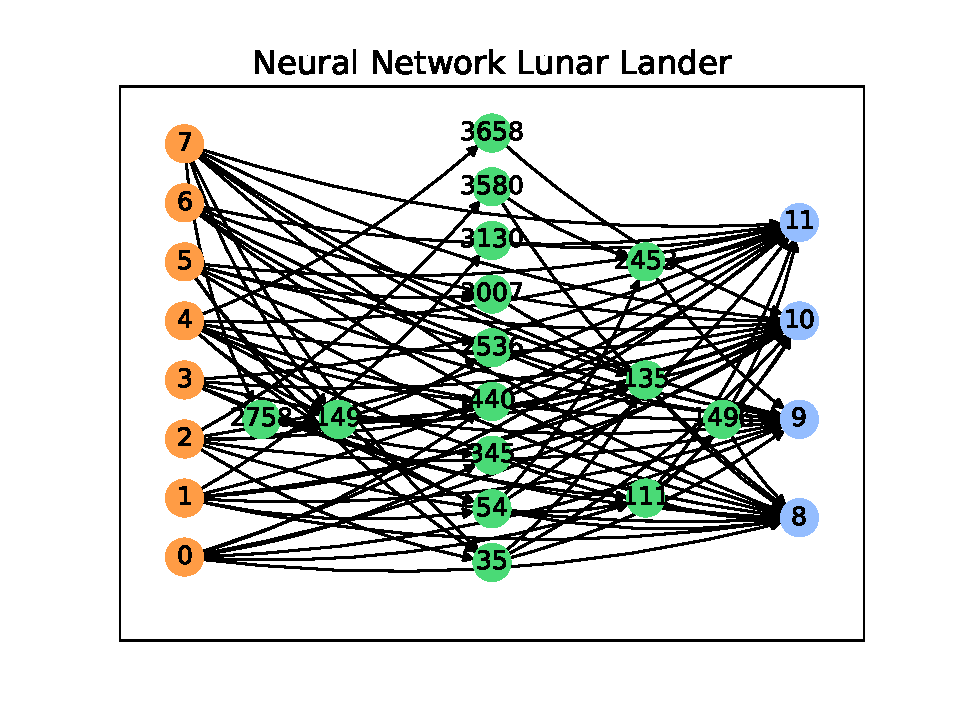
\includegraphics[width=1.0\textwidth]{./img/lunar_lander/lunar_lander_network.pdf} 
	\end{minipage}
	\hfill
	\begin{minipage}[]{0.49\textwidth}
		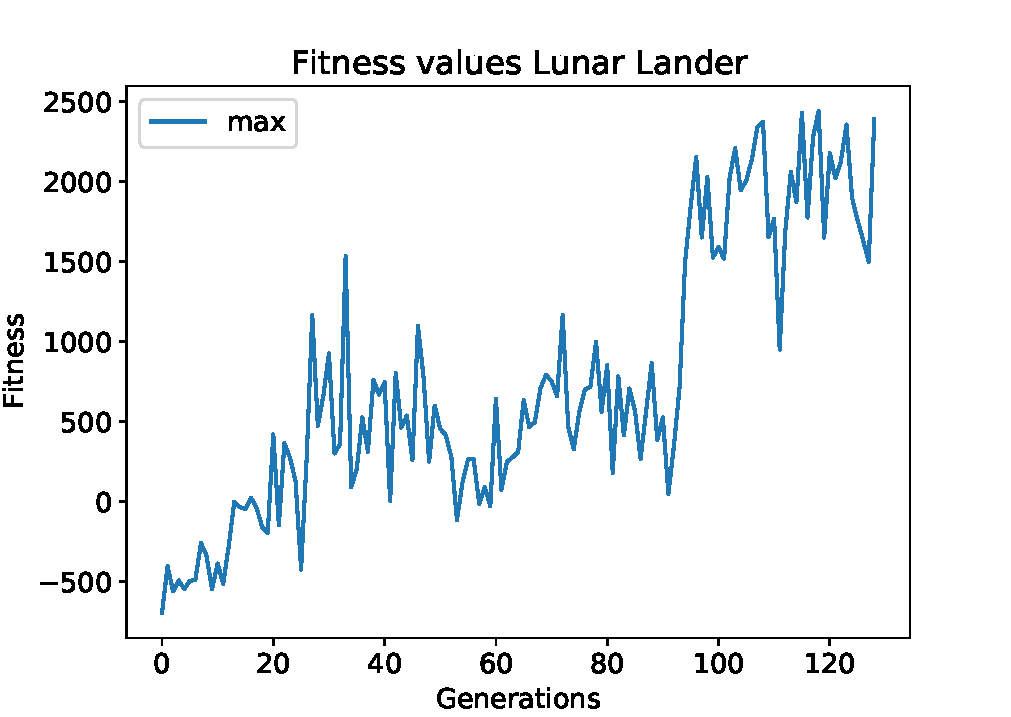
\includegraphics[width=1.0\textwidth]{./img/lunar_lander/lunar_lander_fitness.pdf} 
	\end{minipage}
	\caption{Links die Lösung für das \emph{Lunar Lander} Problem, rechts die dazugehörigen Fitnesswerte pro Generation}
	\label{fig:lunar_lander_neural_network_and_fitness}
\end{figure}
Abbildung \ref{fig:lunar_lander_neural_network_and_fitness} zeigt das finale \ac{KNN} und den Verlauf des maximalen Fitnesswertes. Das \ac{KNN} hat $15$ \emph{Hidden}-Neuronen entwickelt und besitzt insgesamt $88$ Verbindungen. Die Fitnesswerte ist anfänglich negativ, da das Raumschiff häufig abstürzt. Im weiteren Verlauf steigt der Fitnesswert zwar an, zeigt aber große Schwankungen durch eine verrauschte Fitnessfunktion. Der Grund hierfür ist, dass nur ein Teil der Startzustände und nicht alle evaluiert werden. So kann ein Agent hohe Fitnesswerte auf Basis günstiger Startpositionen erhalten, wie es beispielsweise in Generation $33$ vorkommt. Dort hat der beste Agent einen Fitnesswert von $1533$ erzielt und obwohl er unverändert in die nächste Generation kopiert wird, sinkt der maximale Fitnesswert in dieser auf $88$ Punkte ab. In Generation $94$ wird ein große Steigerung des Fitnesswertes auf $1495$ Punkte erzielt. Letztendlich endet das Verfahren nach 128 Generationen und einem Fitnesswert von $2394$. Eine Besonderheit ist, dass der maximale Fitnesswert von $2441$ Punkten nicht am Ende des Verfahrens sondern in Generation $118$ erzielt wird. Aber da die Abbruchbedingungen nicht erfüllt ist, wird das Verfahren fortgeführt. Bei der Visualisierung des final entwickelten \ac{KNN} zeigt sich, dass das Verfahren grundsätzlich erfolgreich ist. Der Agent landet in vielen Fällen direkt auf der Zielplattform und erreicht Fitnesswerte zwischen $240$ bis $280$ Punkten. Allerdings gibt es auch Durchläufe in denen der Agent abdriftet. In diesen Fällen landet das Raumschiff nicht auf der Plattform, dennoch werden Fitnesswerte um die $200$ Punkte erreicht. Insgesamt hat das Optimierungsverfahren eine generelle Lösungsstrategie entwickelt, aber die erreichten Fitnesswerte können durch die unterschiedlichen Startpositionen trotzdem abweichen. Eine noch bessere Leistung kann durch die Evaluation von weiteren Startzuständen oder eine höhere Trainingszeit erreicht werden.
\begin{figure}[!h]
	\centering
	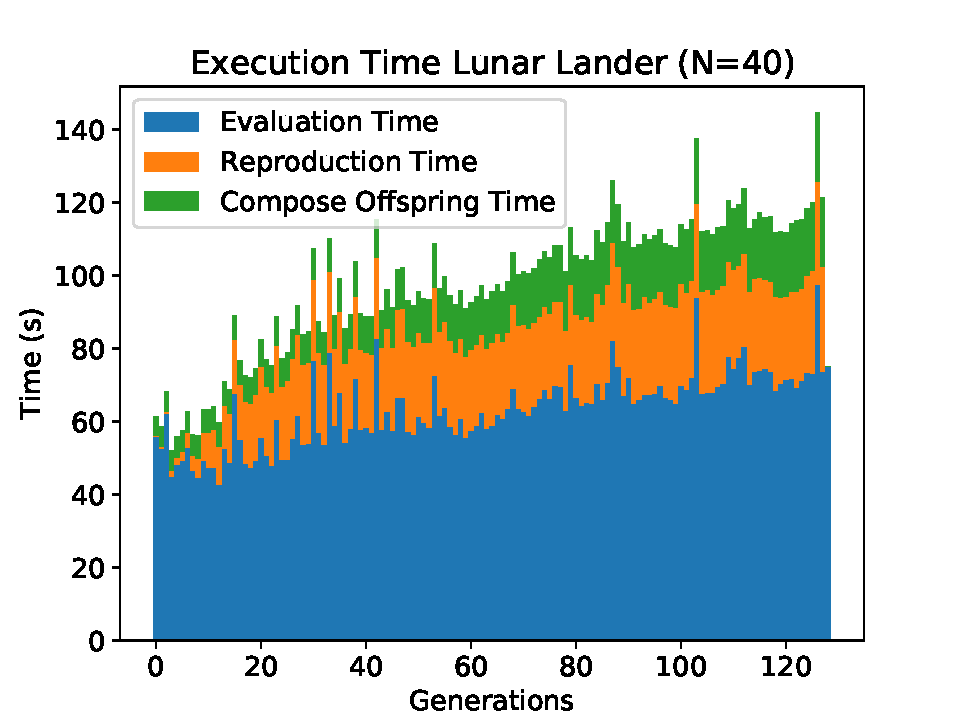
\includegraphics[width=0.7\textwidth]{./img/lunar_lander/lunar_lander_time_40.pdf} 
	\caption{Ausführungszeit des \emph{Lunar Lander} Problems auf 10 \emph{Raspberry Pis} mit 40 Prozessen}
	\label{fig:lunar_lander_time_40core_10pi}
\end{figure}
\\\\
Abbildung \ref{fig:lunar_lander_time_40core_10pi} zeigt die gemessenen Ausführungszeiten mit $40$ Prozessen auf zehn Raspberry Pis. Insgesamt hat das Verfahren etwa $3.5$ Stunden benötigt. Hiervon werden ungefähr $65\%$ für die \emph{Evaluation Time} verwendet. Der zweit größte Faktor bei der Ausführungszeit ist die \emph{Reproduction Time} mit ungefähr $22\%$, welcher wie bei der \emph{Pendulum} Umgebung durch viele verschiedene Spezies zu erklären ist. Wie bei der \emph{Mountain Car} Umgebung, unterliegt die Ausführungszeit der einzelnen Generationen einigen Schwankungen, da die Evaluationszeit je nach Agenten stark abweichen kann. Stürzt das Raumschiff direkt ab oder landet schnell, ist die Evaluationszeit kurz. Evaluationen mit einer hohen Flugzeit hingegen, können vergleichsweise lang andauern. Auch die Größte des \ac{KNN} kann eine entscheidender Faktor sein. Sowohl bei der \emph{Evaluation} als auch in den Phasen \emph{Mutation} und \emph{Rekombination}. Um in solchen Szenarien gute Effizienzwerte zu erhalten, ist die dynamische Zuteilung von Arbeitspaketen durch die \emph{Master-Slave} Architektur besonders wichtig. Prinzipiell hätte diese Umgebung auch in Kapitel \ref{chap:analysis} bei der Analyse verwendet werden können, allerdings ist die lange Ausführungszeit unpraktikabel. Mit den \emph{SpeedUp} Werten aus der \emph{Mountain Car} und \emph{Pendulum} Umgebung ist auf die sequenzielle Ausführungszeit zu schließen. Bei einem \emph{SpeedUp} Faktor von $26.7$ liegt die erwartete Ausführungszeit auf einem Prozess bei $62,1$ Stunden und mit einem Faktor von $29.6$ bei $68.7$ Stunden. 